\documentclass[]{article}
\usepackage{lmodern}
\usepackage{amssymb,amsmath}
\usepackage{ifxetex,ifluatex}
\usepackage{fixltx2e} % provides \textsubscript
\ifnum 0\ifxetex 1\fi\ifluatex 1\fi=0 % if pdftex
  \usepackage[T1]{fontenc}
  \usepackage[utf8]{inputenc}
\else % if luatex or xelatex
  \ifxetex
    \usepackage{mathspec}
  \else
    \usepackage{fontspec}
  \fi
  \defaultfontfeatures{Ligatures=TeX,Scale=MatchLowercase}
\fi
% use upquote if available, for straight quotes in verbatim environments
\IfFileExists{upquote.sty}{\usepackage{upquote}}{}
% use microtype if available
\IfFileExists{microtype.sty}{%
\usepackage{microtype}
\UseMicrotypeSet[protrusion]{basicmath} % disable protrusion for tt fonts
}{}
\usepackage[margin=1in]{geometry}
\usepackage{hyperref}
\hypersetup{unicode=true,
            pdfborder={0 0 0},
            breaklinks=true}
\urlstyle{same}  % don't use monospace font for urls
\usepackage{natbib}
\bibliographystyle{apalike}
\usepackage{longtable,booktabs}
\usepackage{graphicx,grffile}
\makeatletter
\def\maxwidth{\ifdim\Gin@nat@width>\linewidth\linewidth\else\Gin@nat@width\fi}
\def\maxheight{\ifdim\Gin@nat@height>\textheight\textheight\else\Gin@nat@height\fi}
\makeatother
% Scale images if necessary, so that they will not overflow the page
% margins by default, and it is still possible to overwrite the defaults
% using explicit options in \includegraphics[width, height, ...]{}
\setkeys{Gin}{width=\maxwidth,height=\maxheight,keepaspectratio}
\IfFileExists{parskip.sty}{%
\usepackage{parskip}
}{% else
\setlength{\parindent}{0pt}
\setlength{\parskip}{6pt plus 2pt minus 1pt}
}
\setlength{\emergencystretch}{3em}  % prevent overfull lines
\providecommand{\tightlist}{%
  \setlength{\itemsep}{0pt}\setlength{\parskip}{0pt}}
\setcounter{secnumdepth}{5}
% Redefines (sub)paragraphs to behave more like sections
\ifx\paragraph\undefined\else
\let\oldparagraph\paragraph
\renewcommand{\paragraph}[1]{\oldparagraph{#1}\mbox{}}
\fi
\ifx\subparagraph\undefined\else
\let\oldsubparagraph\subparagraph
\renewcommand{\subparagraph}[1]{\oldsubparagraph{#1}\mbox{}}
\fi

%%% Use protect on footnotes to avoid problems with footnotes in titles
\let\rmarkdownfootnote\footnote%
\def\footnote{\protect\rmarkdownfootnote}

%%% Change title format to be more compact
\usepackage{titling}

% Create subtitle command for use in maketitle
\newcommand{\subtitle}[1]{
  \posttitle{
    \begin{center}\large#1\end{center}
    }
}

\setlength{\droptitle}{-2em}
  \title{}
  \pretitle{\vspace{\droptitle}}
  \posttitle{}
  \author{}
  \preauthor{}\postauthor{}
  \date{}
  \predate{}\postdate{}

\usepackage{booktabs}
% \usepackage{xcolor}
\usepackage{amsthm}
\usepackage{float}
\usepackage[utf8]{inputenc}
\usepackage[brazil]{babel}
\usepackage[table]{xcolor}
\usepackage{eso-pic}
\newcommand\BackgroundPic{%
\put(0,0){%
\parbox[b][\paperheight]{\paperwidth}{%
\vfill
\centering
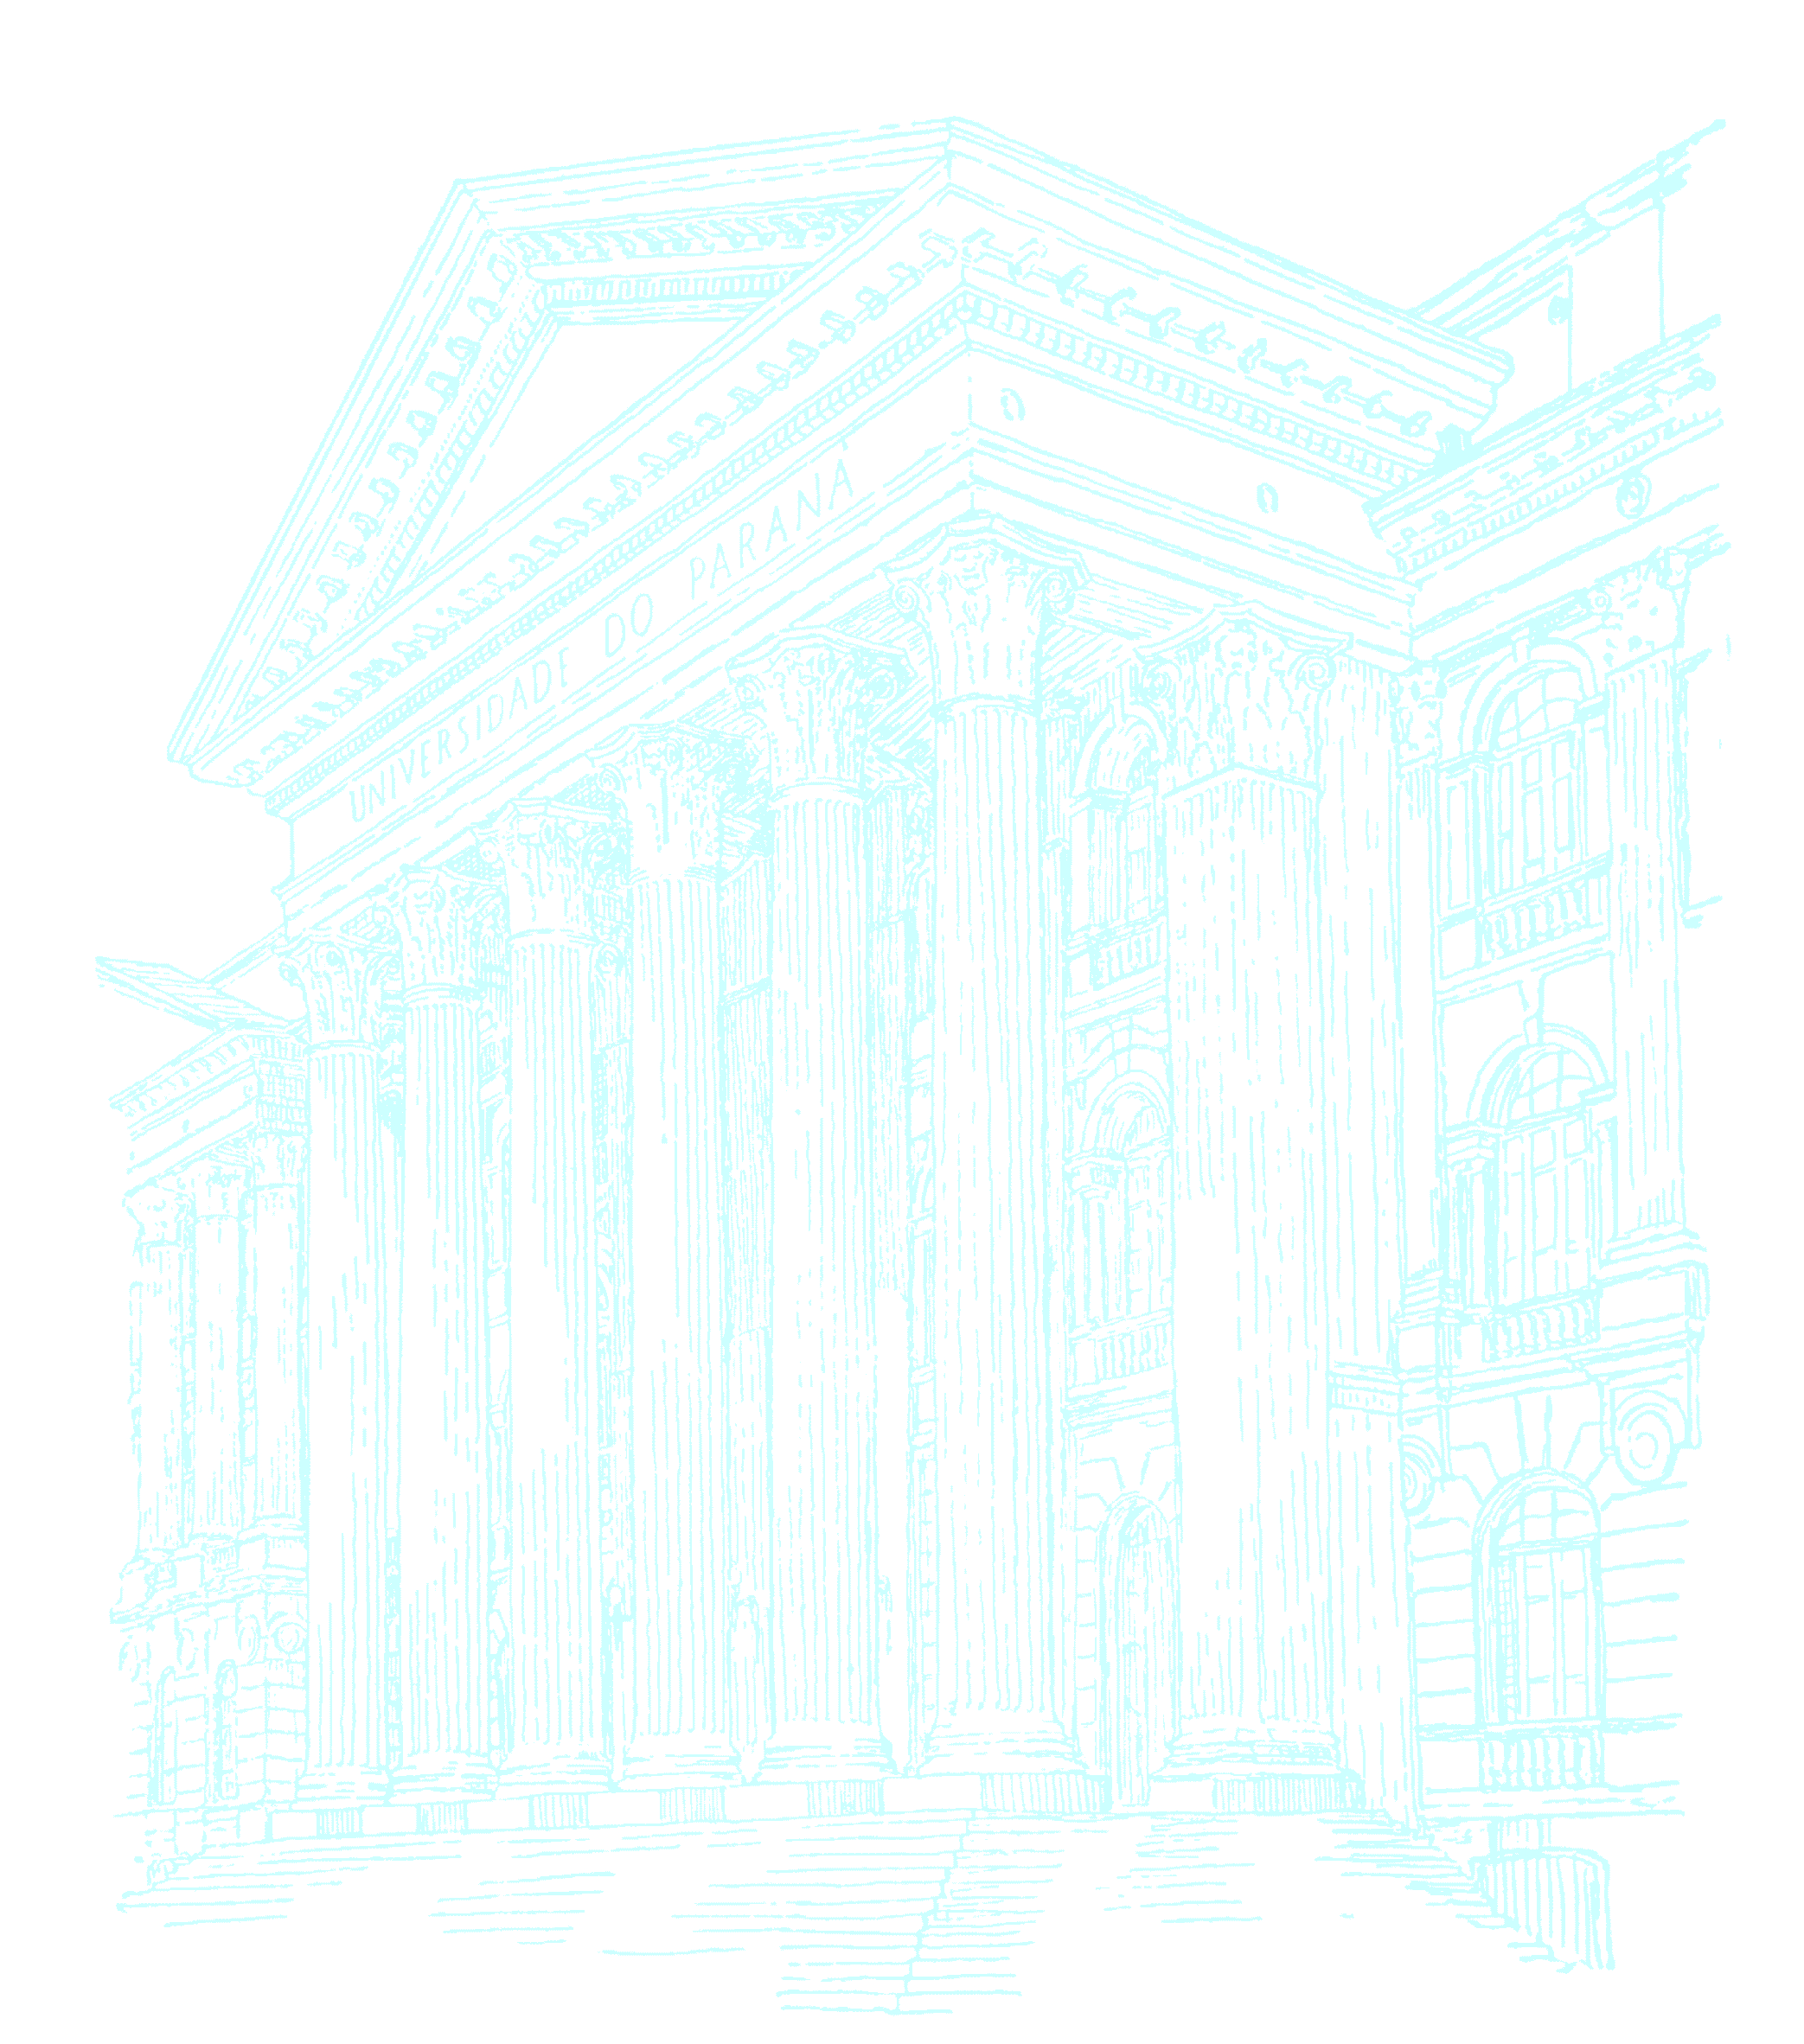
\includegraphics[width=\paperwidth,height=\paperheight,%
keepaspectratio]{ufpr.jpg}%
\vfill
}}}
\AddToShipoutPicture*{\BackgroundPic}

\begin{document}

\begin{titlepage}
\centering{\large{UNIVERSIDADE FEDERAL DO PARANÁ}}
\\
\centering{Departamento de Estatística}

\vspace{7.5cm}

\centering{\huge{OPERAÇÃO LAVA JATO TRI}}

\vspace{3cm}

CE095 - Teorias de Avalição

\vspace{2cm}

Andryas Waurzenczak, GRR: 20149125 \\
Gabriel Sartori, GRR: 20124671


\vfill

07/06/2018
\end{titlepage}


\begin{abstract}
Abstract
\end{abstract}


\pagebreak
\tableofcontents
\pagebreak

O presente trabalho é fruto dos esforços da turma do 1º semestre de 2018
do curso de Teorias de Avaliação ministrada pelo professor
\href{}{Adilson dos Anjos}.

\section{Introdução}\label{introducao}

A Política é um tema bastante debatido nos mais diversos lugares, seja
nas universidades, bares, televisão, etc \ldots{} isto porque ela
interessa a todos nós. Dito isso, o presente trabalho é uma tentativa de
quantificar o quanto nossos amigos, amigos de nossos amigos, familiares
e pessoas ao nosso redor estão atualizados/informados sobre a política
atual do Brasil.

Para tal quantificação selecionamos um tema recente e que tem tido muita
repercusão. O assunto é a \textbf{Operaçao Lava Jato}, que é um conjunto
de investigações ainda em andamento pela Polícia Federal do Brasil, que
começou em 17 de março de 2014.

\section{Materiais e Métodos}\label{materiais-e-metodos}

O materias e métodos são descritos a seguir.

\subsection{Materiais}\label{materiais}

O conjunto de dados é um produto dos esforços da turma de Teorias de
Avaliação, 1º semestre de 2018, com uma pequena contribuição da turma
passada. A forma de coleta se deu atráves de um formulario online que
ficou disponivel na plataforma do
\href{https://www.google.com/forms/about/}{Google} por 21 dias.

O desenvolvimento do questinário foi feito em 5 etapas.

\begin{enumerate}
\def\labelenumi{\arabic{enumi}.}
\tightlist
\item
  Elaboração dos itens
\item
  Validação dos itens
\item
  Seleção dos itens
\item
  Elaboração de Fatores Associados
\item
  Disponibilização do formulário
\end{enumerate}

Para a execução da 1ª e 2ª etapa utilizou-se como embasamento o
\href{www.ufpr.br/~aanjos/CE095/guia_elaboracao_revisao_itens_2012_INEP.pdf}{guia
de elaboração de revisão de itens da INEP - 2012}. Cada aluno
desenvolveu 3 questões que foram depois distribuidas de forma aleatoria
para um dos colegas avaliar se o item estava de acordo ou não. A ideia
básica para a criação e validação dos itens era possuir
\textbf{TEXTO-BASE}, \textbf{ENUNCIADO}, \textbf{ALTERNATIVAS} e
\textbf{GABARITO}. Dos itens que passaram dessas 2 primeiras etapas, 20
foram selecionados e foram complementados com mais 6 itens de um
instrumento de medida anterior ao nosso que apresentaram boa calibração.
Ao todo tivemos 26 itens no nosso intrusmento de medida.

Após isso foi elaborado candidatos a fatores associados dos quais foi
escolhido três e então o questionario foi disponibilizado no dia 10 de
Maio de 2018.

O conjunto de dados teve ao todo 568 respondentes. Para informações
sobre o questionário, perguntas e alternativas, consulte o
\protect\hyperlink{Anexo}{Anexo}

\subsection{Métodos}\label{metodos}

Falar os métodos utilizados (descreve-los) Modelo de três parâmetros

\subsection{Recursos Computacionais}\label{recursos-computacionais}

Para as análises o software utilizado foi \citet{software-r} e os
pacotes utilizados foram:

\section{Resultados}\label{resultados}

\subsection{Pré-Processamento}\label{pre-processamento}

Antes de prosseguir para análise descritiva dos dados, houve um
pré-processamento para a limpeza do conjunto de dados. Observou-se que
alguns respondentes deixaram o questionário em branco, por isso para
este estudo indivíduos que deixaram mais de 3 itens sem resposta foram
desconsiderados. Assim o conjunto de dados passou a ter 549 respondetes
que deixaram no máximo 3 questões sem resposta. E esses individuos que
não responderam foi considerado a ausência de resposta como errado.

\subsection{Análise Descritiva}\label{analise-descritiva}

\subsubsection{Fatores Associados}\label{fatores-associados}

Para dar inicio a análise descritiva iniciamos explorando a frequência
dos fatores associados.

\begin{itemize}
\item
  \begin{enumerate}
  \def\labelenumi{\alph{enumi})}
  \tightlist
  \item
    Você procura se informar sobre os principais acontecimentos
    políticos no país?
  \end{enumerate}
\item
  \begin{enumerate}
  \def\labelenumi{\alph{enumi})}
  \setcounter{enumi}{1}
  \tightlist
  \item
    Você participou de alguma manifestação de apoio a Operação Lava
    Jato? Por exemplo: participou de alguma passeata ou protesto, mandou
    mensagens por redes sociais na internet etc.
  \end{enumerate}
\item
  \begin{enumerate}
  \def\labelenumi{\alph{enumi})}
  \setcounter{enumi}{2}
  \tightlist
  \item
    Você mora em Curitiba?
  \end{enumerate}
\end{itemize}

\begin{center}\includegraphics{work_files/figure-latex/plot_fatores_associados-1} \end{center}

Nota-se pelos gráficos acima que não existe nenhuma concentração de
frequências, pode-se dizer que os fatores associados tem boa
variabilidade.

\subsubsection{Frequência de Acertos}\label{frequencia-de-acertos}

Pelo gráfico abaixo pode-se observar a frequência de indíviduos que
acertaram um número determiniado de itens. Tem-se que a concentração da
quantidade de acertos está entre 10 e 17.

\begin{figure}[H]

{\centering \includegraphics{work_files/figure-latex/freq-acertos-1} 

}

\caption{Frequência da quantidade de acertos}\label{fig:freq-acertos}
\end{figure}

\subsubsection{Alpha de Cronbach}\label{alpha-de-cronbach}

Para verificar a consistência internar do instrumento foi calculado o
\emph{Alpha de Cronbach}.

\[\alpha = 0.75\]

Utilizando como referência \citet{landis}, tem-se que o Alpha de
Cronbach apresentou um valor substâncial de consistência interna do
instrumento.

\subsection{Modelo de três Parâmetros}\label{modelo-de-tres-parametros}

Para este trabalho foi considerado o modelo de três parâmetros e foi
excluido itens que tiveram estimativas dos parâmetros de dificuldade e
discriminação que não estivessem nos seguintes intervalos:

\[-3.5 < \text{Dificuldade} < 3.5\] \[0.6 < \text{Discriminacao} < 3\]

ressalta-se que os intervalos acima sugeridos não foram rigorosos, na
literatura recomenda-se \textbf{-3 \textless{} Dificuldade \textless{}
3} e \textbf{0.8 \textless{} Discriminação \textless{} 3}.

Assim, foram removidos os seguintes itens:

i2, i4, i7, i10, i13, i15, i18, i22, i23, i24, i26

\subsubsection{Estimativas do Modelo}\label{estimativas-do-modelo}

\subsubsection{Informação dos itens}\label{informacao-dos-itens}

\begin{center}\includegraphics{work_files/figure-latex/unnamed-chunk-1-1} \end{center}

\subsubsection{Informação do teste}\label{informacao-do-teste}

\begin{center}\includegraphics{work_files/figure-latex/unnamed-chunk-2-1} \end{center}

\subsubsection{\texorpdfstring{Traço Latente
(\(\theta\))}{Traço Latente (\textbackslash{}theta)}}\label{traco-latente-theta}

\begin{table}[!h]

\caption{\label{tab:tab-traço-latente1}6 Primeiras linhas}
\centering
\begin{tabular}[t]{rrrrrr}
\toprule
\multicolumn{3}{c}{Ordenado por Acerto} & \multicolumn{3}{c}{Ordenado por Escore} \\
\cmidrule(l{2pt}r{2pt}){1-3} \cmidrule(l{2pt}r{2pt}){4-6}
Escore & Posição & Acertos & Escore & Posição & Acertos\\
\midrule
-2.114254 & 546 & 1 & -2.273214 & 549 & 1\\
-2.273214 & 549 & 1 & -2.208348 & 548 & 2\\
-1.805793 & 539 & 2 & -2.183557 & 547 & 2\\
-1.874027 & 541 & 2 & -2.114254 & 546 & 1\\
-1.510591 & 526 & 2 & -2.047984 & 545 & 2\\
-2.047984 & 545 & 2 & -2.003385 & 544 & 2\\
\bottomrule
\end{tabular}
\end{table}

\begin{table}[!h]

\caption{\label{tab:tab-traço-latente2}6 Últimas linhas}
\centering
\begin{tabular}[t]{rrrrrr}
\toprule
\multicolumn{3}{c}{Ordenado por Acerto} & \multicolumn{3}{c}{Ordenado por Escore} \\
\cmidrule(l{2pt}r{2pt}){1-3} \cmidrule(l{2pt}r{2pt}){4-6}
Escore & Posição & Acertos & Escore & Posição & Acertos\\
\midrule
1.978415 & 4 & 15 & 1.978415 & 4 & 15\\
1.978415 & 4 & 15 & 1.978415 & 4 & 15\\
1.978415 & 4 & 15 & 1.978415 & 4 & 15\\
1.978415 & 4 & 15 & 1.978415 & 4 & 15\\
1.978415 & 4 & 15 & 1.978415 & 4 & 15\\
1.978415 & 4 & 15 & 1.978415 & 4 & 15\\
\bottomrule
\end{tabular}
\end{table}

\subsubsection{Interpretação da Escala}\label{interpretacao-da-escala}

\begin{figure}[H]

{\centering \includegraphics{work_files/figure-latex/itemancoras-1} 

}

\caption{Itens Âncoras}\label{fig:itemancoras}
\end{figure}

Os seguintes itens foram ancoras\ldots{}.

\subsection{Análise dos Fatores
Associados}\label{analise-dos-fatores-associados}

\begin{verbatim}
## 
## Call:
## lm(formula = theta ~ ., data = tfatores)
## 
## Residuals:
##     Min      1Q  Median      3Q     Max 
## -2.4547 -0.4889 -0.0157  0.5049  2.6276 
## 
## Coefficients:
##              Estimate Std. Error t value Pr(>|t|)    
## (Intercept)   -0.1739     0.0555   -3.13   0.0018 ** 
## X1Sempre.      0.6015     0.0717    8.39  4.3e-16 ***
## X1Raramente.  -0.5908     0.0916   -6.45  2.5e-10 ***
## X1Nunca.      -0.7300     0.1834   -3.98  7.8e-05 ***
## X2Sim.         0.2112     0.0697    3.03   0.0026 ** 
## X3Não.         0.0435     0.0632    0.69   0.4919    
## ---
## Signif. codes:  0 '***' 0.001 '**' 0.01 '*' 0.05 '.' 0.1 ' ' 1
## 
## Residual standard error: 0.73 on 541 degrees of freedom
##   (2 observations deleted due to missingness)
## Multiple R-squared:  0.297,  Adjusted R-squared:  0.291 
## F-statistic: 45.8 on 5 and 541 DF,  p-value: <2e-16
\end{verbatim}

\section{Considerações Finais}\label{consideracoes-finais}

\hypertarget{Anexo}{\section{Anexo}\label{Anexo}}

\bibliography{book.bib}


\end{document}
